\chapter{Equilibrio químico: cociente y constante}\label{ch:g12:equilibrium}

Una botella cerrada de agua con gas conserva sus burbujas durante meses;
abierta, se queda sin gas en una tarde. En ninguno de los dos casos ha
ido nada mal. En la botella cerrada, el dióxido de carbono sale del agua
y vuelve a ella al mismo ritmo, y la composición no cambia; al abrir el
tapón, el gas que sale ya no vuelve. Muchas reacciones se comportan así:
se detienen antes de que se agote ningún \omterm{def:g7:chemical-reactions:reactant}{reactivo}, en un equilibrio entre
dos reacciones opuestas. Este capítulo describe ese equilibrio con un
solo número.

\begin{recall}
El avance $x$ de una reacción, su máximo $x_{\max}$ y las \omterm{def:g10:reaction-progress-table:limiting}{reacciones
totales} que lo alcanzan (\cref{ch:g10:reaction-progress-table}). Las
velocidades y los \omterm{def:g12:reaction-rates:kinetic-factor}{factores cinéticos} (\cref{ch:g12:reaction-rates}); un
\omterm{def:g12:catalysis:catalyst}{catalizador} no cambia el \omterm{def:g10:reaction-progress-table:system}{estado final} (\cref{ch:g12:catalysis}).
\end{recall}

\begin{omfigure}
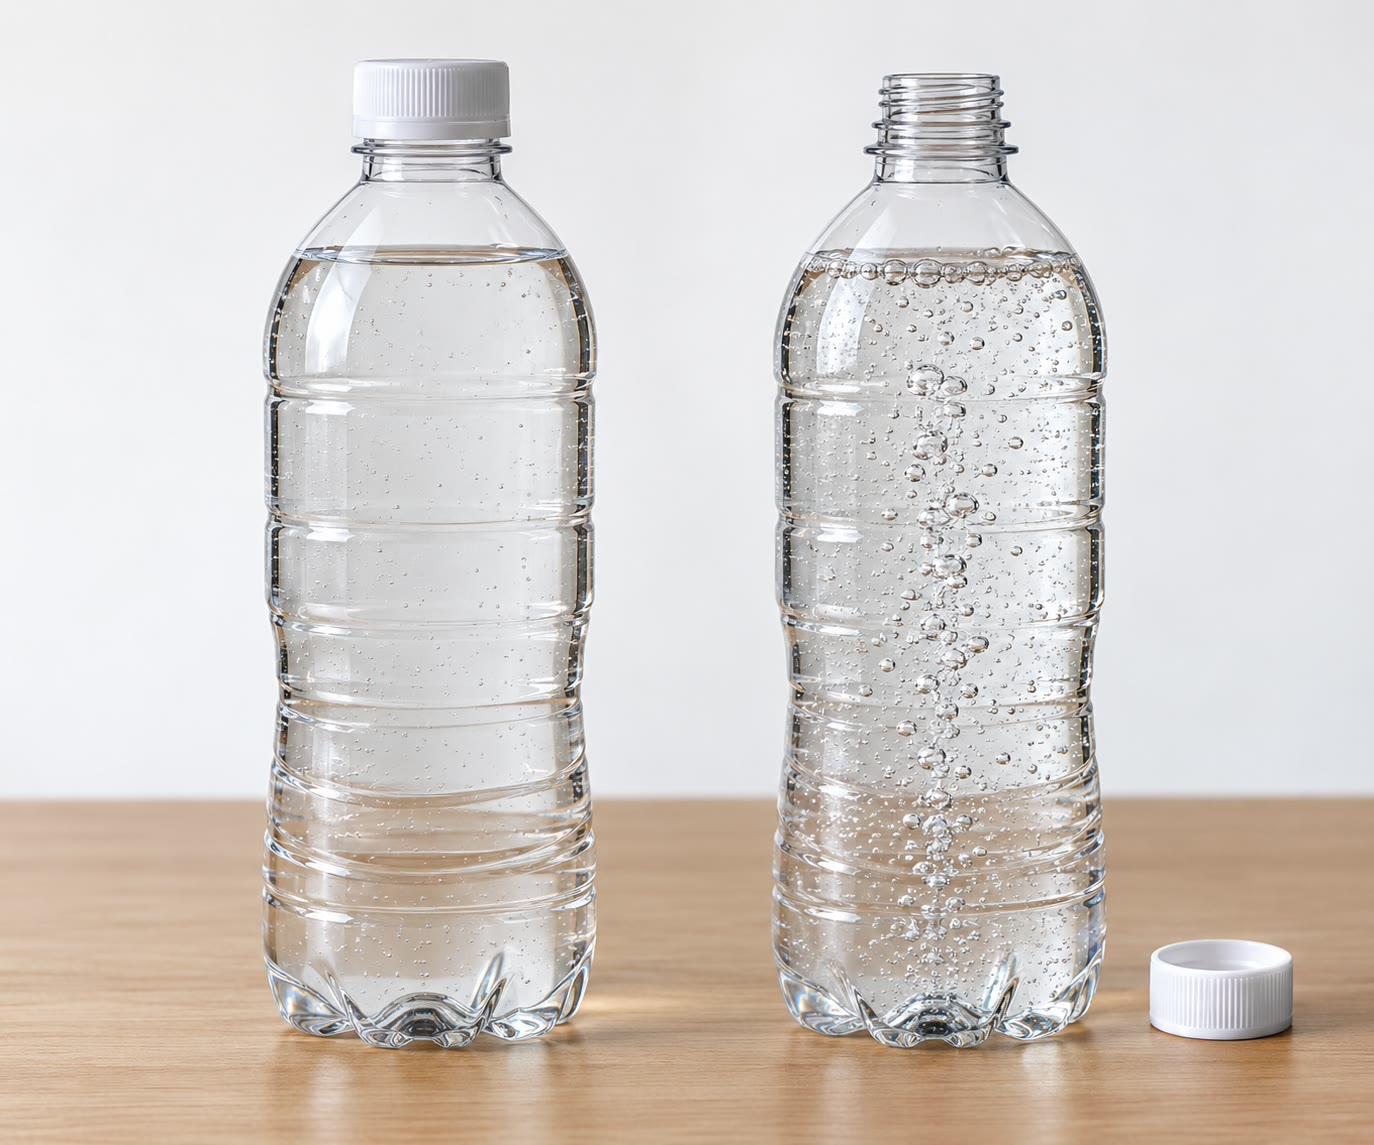
\includegraphics[width=0.45\linewidth,height=5cm,keepaspectratio]{images/book1/ai/g12-fizzy-bottles.jpg}

{\small Cerrada, el agua conserva su gas; abierta, el gas se escapa y no
vuelve.}
\end{omfigure}

\section{Reacciones que no son totales}

\begin{definition}[Reacción no total, tasa de avance final]\label{def:g12:equilibrium:non-total}
Una reacción es una \emph{reacción no total}\index{reaccion no total@reacción no total} si
se detiene en un avance final $x_f$ menor que su \omterm{def:g10:reaction-progress-table:limiting}{avance máximo}
$x_{\max}$, con todos los \omterm{def:g7:chemical-reactions:reactant}{reactivos} todavía presentes. Su \emph{tasa de
avance final}\index{tasa de avance final} es
\[
  \tau = \frac{x_f}{x_{\max}}, \qquad 0 < \tau < 1
\]
($\tau = 1$ para una \omterm{def:g10:reaction-progress-table:limiting}{reacción total}).
\end{definition}

\begin{example}[Un éster que se queda a medio camino]\label{ex:g12:equilibrium:berthelot}
% ledger: ester:berthelot
Calentado con \qty{1}{mol} de etanol, \qty{1}{mol} de ácido etanoico
forma etanoato de etilo y agua,
\ce{CH3COOH + C2H5OH <=> CH3COOC2H5 + H2O}. La reacción se detiene cuando
han reaccionado unos dos tercios del ácido: $x_f = \qty{0.67}{mol}$ para
$x_{\max} = \qty{1}{mol}$, así que $\tau \approx 0.67$. Partiendo de
\qty{1}{mol} de \omterm{def:g11:functional-groups:carboxylic-acid}{éster} y \qty{1}{mol} de agua, la reacción inversa
también se detiene, con alrededor de un tercio del \omterm{def:g11:functional-groups:carboxylic-acid}{éster} hidrolizado: la
misma \omterm{def:g6:pure-substances-and-mixtures:mixture}{mezcla} final.
\end{example}

\begin{history}[Berthelot y Péan de Saint-Gilles, 1862]
% ledger: ester:berthelot
Los químicos Marcellin Berthelot y Léon Péan de Saint-Gilles calentaron
durante largos periodos \omterm{def:g6:pure-substances-and-mixtures:mixture}{mezclas} de ácido etanoico y etanol, y de
etanoato de etilo y agua, y las analizaron. A partir de cantidades
iguales de ácido y de \omterm{def:g11:functional-groups:alcohol}{alcohol}, la reacción siempre se detenía hacia los
dos tercios; a partir de \omterm{def:g11:functional-groups:carboxylic-acid}{éster} y agua, con un tercio de hidrólisis; y
observaron que la cantidad de \omterm{def:g11:functional-groups:carboxylic-acid}{éster} formada en cada momento dependía del
producto de las cantidades de los \omterm{def:g7:chemical-reactions:reactant}{reactivos}. Su trabajo fue uno de los
primeros estudios cuantitativos de un equilibrio químico.
\end{history}

\section{El estado de equilibrio}

\begin{definition}[Estado de equilibrio]\label{def:g12:equilibrium:equilibrium-state}
Un sistema está en un \emph{estado de equilibrio}\index{estado de equilibrio}
cuando su composición ya no cambia aunque la reacción directa y la
inversa siguen produciéndose, a la misma velocidad. Una reacción que
puede alcanzar un estado así se escribe con la doble flecha $\rightleftharpoons$.
\end{definition}

\begin{omfigure}
\begin{tikzpicture}
\begin{axis}[width=0.8\linewidth, height=6cm, xmin=0, xmax=200, ymin=0,
    ymax=1.05, xlabel={$t$ (\si{h})}, ylabel={cantidad de éster (\si{mol})},
    axis lines*=left, ymajorgrids, grid style={gray!20},
    tick label style={font=\small}, label style={font=\small},
    legend style={font=\small, at={(0.98,0.98)}, anchor=north east,
    draw=none, fill=white}, legend cell align=left]
  % ledger: ester:berthelot (K = 4; kinetics synthetic)
  \addplot[very thick, omDef] table[x=t, y=fromAcid] {figdata/out/grade-12-equilibrium.dat};
  \addplot[very thick, omProp] table[x=t, y=fromEster] {figdata/out/grade-12-equilibrium.dat};
  \addplot[dashed, black!60] coordinates {(0,0.6667) (200,0.6667)};
  \legend{desde 1 mol de ácido + 1 mol de alcohol, desde 1 mol de éster + 1 mol de agua}
  \node[font=\small, anchor=north east] at (axis cs:195,0.65) {equilibrio: $\tfrac{2}{3}$ mol};
\end{axis}
\end{tikzpicture}

{\small La esterificación (en azul) y la hidrólisis del \omterm{def:g11:functional-groups:carboxylic-acid}{éster} (en
naranja) alcanzan la misma composición de equilibrio, desde lados
opuestos. (La escala de tiempo es un modelo; el valor final es el
medido.)}
\end{omfigure}

\section{El cociente de reacción}

\begin{notation}[Concentración estándar]\label{not:g12:equilibrium:c-standard}
$c^\circ = \qty{1}{mol/L}$ es la concentración estándar. Dividir una
concentración por $c^\circ$ da un número sin unidad con el mismo valor:
$[\ce{A}]/c^\circ$.
\end{notation}

\begin{definition}[Cociente de reacción]\label{def:g12:equilibrium:quotient}
Para una reacción en disolución $a\,\ce{A} + b\,\ce{B} \rightleftharpoons c\,\ce{C} + d\,\ce{D}$, el \emph{cociente
de reacción}\index{cociente de reaccion@cociente de reacción} en un estado dado del sistema es
\[
  Q = \frac{\left([\ce{C}]/c^\circ\right)^c \left([\ce{D}]/c^\circ\right)^d}
           {\left([\ce{A}]/c^\circ\right)^a \left([\ce{B}]/c^\circ\right)^b} .
\]
Los sólidos, y el \omterm{def:g6:solutions-and-solubility:solute}{disolvente} (el agua en una \omterm{def:g6:solutions-and-solubility:solute}{disolución acuosa}), no
aparecen en $Q$.
\end{definition}


\begin{example}[Escribir cocientes]\label{ex:g12:equilibrium:quotients}
Para \ce{CH3COOH + H2O <=> CH3COO- + H3O+} en agua (el \omterm{def:g9:ions:ion}{ion} \ce{H3O+} se
presenta en el capítulo siguiente), el agua es el \omterm{def:g6:solutions-and-solubility:solute}{disolvente}:
$Q = \dfrac{[\ce{CH3COO-}]\,[\ce{H3O+}]}{[\ce{CH3COOH}]\,c^\circ}$. Para
la disolución de un sólido, \ce{AgCl(s) <=> Ag+ + Cl-}, el sólido no se
incluye: $Q = [\ce{Ag+}][\ce{Cl-}]/(c^\circ)^2$. Para la esterificación,
en la que las cuatro especies están en la misma \omterm{def:g6:pure-substances-and-mixtures:mixture}{mezcla} líquida de
volumen $V$, los volúmenes se simplifican y $Q = \dfrac{n_{\text{éster}}\, n_{\text{agua}}}{n_{\text{ácido}}\, n_{\text{alcohol}}}$.
\end{example}

\section{La constante de equilibrio}

\begin{definition}[Constante de equilibrio]\label{def:g12:equilibrium:constant}
El valor $Q_{eq}$ del \omterm{def:g12:equilibrium:quotient}{cociente de reacción} en el \omterm{def:g12:equilibrium:equilibrium-state}{estado de equilibrio} es
la \emph{constante de equilibrio}\index{constante de equilibrio} $K$ de
la reacción. No tiene unidad.
\end{definition}

\begin{proposition}[$K$ solo depende de la temperatura]\label{prop:g12:equilibrium:constant}
Para una reacción dada, $Q_{eq} = K$ en todo \omterm{def:g12:equilibrium:equilibrium-state}{estado de equilibrio} a una
temperatura dada, sean cuales sean las cantidades iniciales.
\end{proposition}

\begin{proof}
Se admite; se deduce en el volumen del segundo año. Se comprueba en la
esterificación: los dos ensayos de la figura, iniciados desde lados
opuestos, dan el mismo $Q_{eq}$.
\end{proof}

\begin{example}[La $K$ de la esterificación]\label{ex:g12:equilibrium:k-ester}
% ledger: ester:berthelot
A partir de \qty{1}{mol} de ácido y \qty{1}{mol} de \omterm{def:g11:functional-groups:alcohol}{alcohol}, el
equilibrio contiene $\frac{2}{3}$ mol de \omterm{def:g11:functional-groups:carboxylic-acid}{éster} y de agua y $\frac{1}{3}$
mol de ácido y de \omterm{def:g11:functional-groups:alcohol}{alcohol}:
\[
  K = \frac{(2/3)\times(2/3)}{(1/3)\times(1/3)} = 4 .
\]
\end{example}

\begin{method}[Estado final de una reacción no total]\label{met:g12:equilibrium:final}
\begin{enumerate}
  \item Completa la \omterm{def:g10:reaction-progress-table:extent}{tabla de avance} con el avance final desconocido
        $x_f$.
  \item Escribe $Q_{eq}$ en función de $x_f$ e iguálalo a $K$.
  \item Despeja $x_f$ (a menudo una ecuación de segundo grado),
        quedándote con la raíz comprendida entre 0 y $x_{\max}$.
  \item Deduce las cantidades finales y $\tau = x_f/x_{\max}$.
\end{enumerate}
\end{method}

\begin{example}[Un exceso de alcohol]\label{ex:g12:equilibrium:excess}
Con \qty{1}{mol} de ácido y \qty{2}{mol} de \omterm{def:g11:functional-groups:alcohol}{alcohol}:
$\dfrac{x^2}{(1-x)(2-x)} = 4$, es decir, $3x^2 - 12x + 8 = 0$, cuya raíz
entre 0 y 1 es $x_f = \qty{0.845}{mol}$. Duplicar el \omterm{def:g11:functional-groups:alcohol}{alcohol} eleva el
\omterm{def:g10:synthesis-yield:yield}{rendimiento}, calculado respecto al ácido, del \qty{67}{\percent} al
\qty{85}{\percent}.
\end{example}

\section{Predecir y desplazar la evolución}

\begin{proposition}[Sentido de evolución]\label{prop:g12:equilibrium:direction}
Si $Q < K$, el sistema evoluciona en sentido directo (los productos
aumentan) hasta que $Q = K$; si $Q > K$, evoluciona en sentido inverso;
si $Q = K$, está en equilibrio y no cambia.
\end{proposition}

\begin{proof}
Se admite: $Q$ aumenta cuando avanza la reacción directa (los productos
del numerador crecen, los \omterm{def:g7:chemical-reactions:reactant}{reactivos} del denominador disminuyen), y el
sistema se dirige hacia el estado en el que $Q = K$.
\end{proof}

\begin{omfigure}
\begin{tikzpicture}[font=\small]
  \draw[->, thick] (0,0) -- (10,0) node[right] {$Q$};
  \draw[thick] (0,-0.12) -- (0,0.12) node[above] {0};
  \draw[very thick, omThm] (5,-0.25) -- (5,0.25) node[above] {$K$};
  \draw[->, very thick, omDef] (1.2,0.55) -- (4.4,0.55);
  \node[omDef, align=center] at (2.8,1.15) {$Q < K$: directo};
  \draw[->, very thick, omProp] (8.8,0.55) -- (5.6,0.55);
  \node[omProp, align=center] at (7.2,1.15) {$Q > K$: inverso};
  \node[align=center] at (5,-0.75) {$Q = K$: equilibrio};
\end{tikzpicture}

{\small El cociente siempre se desplaza hacia la constante.}
\end{omfigure}

\begin{remark}[Desplazar un equilibrio]\label{rem:g12:equilibrium:shift}
Para obtener más producto de una \omterm{def:g12:equilibrium:non-total}{reacción no total}, se puede añadir un
exceso de uno de los \omterm{def:g7:chemical-reactions:reactant}{reactivos} (el más barato), o retirar un producto a
medida que se forma: en ambos casos vuelve a ser $Q < K$, y el sistema
avanza en sentido directo. Retirar el agua de una esterificación (con un
agente desecante, o destilándola) puede llevar la reacción casi hasta el
final. La botella abierta de agua con gas hace lo mismo con el dióxido
de carbono que se escapa.
\end{remark}

\begin{omfigure}
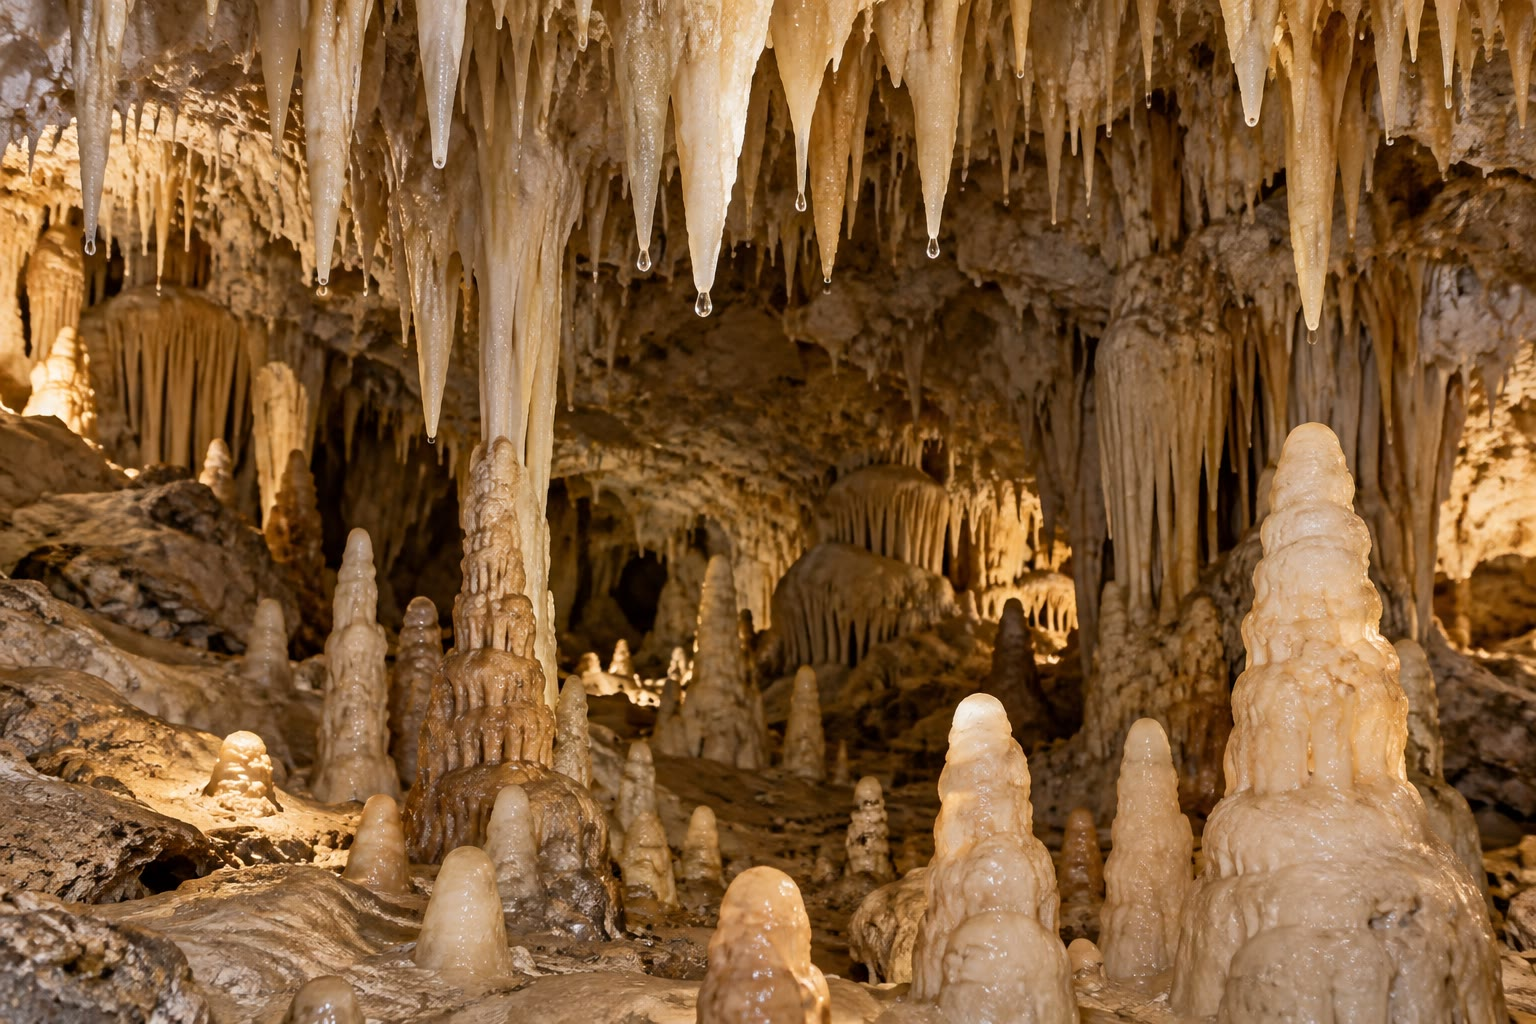
\includegraphics[width=0.45\linewidth]{images/book1/ai/g12-cave-stalactites.jpg}

{\small Las estalactitas crecen donde el agua que gotea en una cueva
cede dióxido de carbono al \omterm{def:g4:air-a-mixture-of-gases:air}{aire}: se desplaza un equilibrio de la caliza
disuelta y se deposita carbonato de calcio.}
\end{omfigure}

\section{Ejercicios}

\begin{exercise}[$\star$]\label{exo:g12:equilibrium:1}
Escribe el \omterm{def:g12:equilibrium:quotient}{cociente de reacción} de: (a) \ce{N2 + 3H2 <=> 2NH3} (gases,
usa concentraciones); (b) \ce{CH3COOH + H2O <=> CH3COO- + H3O+} en agua;
(c) \ce{CaCO3(s) <=> Ca^{2+} + CO3^{2-}}; (d) \ce{Fe^{3+} + SCN- <=>
FeSCN^{2+}}.
\end{exercise}

\begin{exercise}[$\star$]\label{exo:g12:equilibrium:2}
Una reacción tiene $x_{\max} = \qty{0.050}{mol}$ y alcanza
$x_f = \qty{0.020}{mol}$. Calcula $\tau$. ¿Es total la reacción?
\end{exercise}

\begin{exercise}[$\star$]\label{exo:g12:equilibrium:3}
Para una reacción con $K = 10$, ¿en qué sentido evoluciona una \omterm{def:g6:pure-substances-and-mixtures:mixture}{mezcla} si
$Q = 2$? ¿Y si $Q = 50$? ¿Y si $Q = 10$?
\end{exercise}

\begin{exercise}[$\star$]\label{exo:g12:equilibrium:4}
Explica por qué se dice que un equilibrio es ``dinámico''.
\end{exercise}

\begin{exercise}[$\star$]\label{exo:g12:equilibrium:5}
¿Cambia un \omterm{def:g12:catalysis:catalyst}{catalizador} el valor de $K$? ¿Y el tiempo necesario para
alcanzar el equilibrio? Explícalo.
\end{exercise}

\begin{exercise}[$\star\star$]\label{exo:g12:equilibrium:6}
Se \omterm{def:g2:mixing-and-dissolving:mix}{mezclan} \qty{2.0}{mol} de ácido etanoico y \qty{2.0}{mol} de etanol
($K = 4$). Calcula las cantidades finales de las cuatro especies.
\end{exercise}

\begin{exercise}[$\star\star$]\label{exo:g12:equilibrium:7}
Una \omterm{def:g6:pure-substances-and-mixtures:mixture}{mezcla} contiene \qty{0.5}{mol} de cada una de estas especies: ácido
etanoico, etanol, etanoato de etilo y agua. Calcula $Q$. ¿En qué sentido
evoluciona?
\end{exercise}

\begin{exercise}[$\star\star$]\label{exo:g12:equilibrium:8}
Con la figura de los dos ensayos, lee la cantidad de \omterm{def:g11:functional-groups:carboxylic-acid}{éster} al cabo de
\qty{20}{h} en cada ensayo. ¿Cuándo puede considerarse que el sistema
está en equilibrio?
\end{exercise}

\begin{exercise}[$\star\star$]\label{exo:g12:equilibrium:9}
Partiendo de \qty{1}{mol} de \omterm{def:g11:functional-groups:carboxylic-acid}{éster} y \qty{1}{mol} de agua ($K = 4$ para
la esterificación, luego $1/4$ para la hidrólisis), calcula las
cantidades finales con el método del capítulo y compáralas con el ensayo
de esterificación.
\end{exercise}

\begin{exercise}[$\star\star$]\label{exo:g12:equilibrium:10}
¿Por qué el sólido no aparece en el cociente de
\ce{AgCl(s) <=> Ag+ + Cl-}? ¿Desplaza el equilibrio añadir más sólido?
\end{exercise}

\begin{exercise}[$\star\star$]\label{exo:g12:equilibrium:11}
En una botella cerrada de agua con gas, el dióxido de carbono sale del
agua y entra en ella al mismo ritmo. Escribe el equilibrio
\ce{CO2(aq) <=> CO2(g)} y explica, con $Q$ y $K$, por qué el agua se
queda sin gas al abrir la botella.
\end{exercise}

\begin{exercise}[$\star\star\star$]\label{exo:g12:equilibrium:12}
Una esterificación de \qty{1}{mol} de ácido y \qty{1}{mol} de \omterm{def:g11:functional-groups:alcohol}{alcohol}
alcanza el equilibrio. Después se retira la mitad del agua presente.
Calcula el nuevo $Q$, di en qué sentido evoluciona el sistema y halla la
nueva cantidad final de \omterm{def:g11:functional-groups:carboxylic-acid}{éster}.
\end{exercise}

\begin{exercise}[$\star\star\star$]\label{exo:g12:equilibrium:13}
Demuestra que la constante de la reacción inversa es $1/K$. ¿Cuál es la
constante de la hidrólisis del etanoato de etilo?
\end{exercise}

\begin{exercise}[$\star\star\star$]\label{exo:g12:equilibrium:14}
Un químico \omterm{def:g6:pure-substances-and-mixtures:mixture}{mezcla} \qty{1}{mol} de ácido, \qty{1}{mol} de \omterm{def:g11:functional-groups:alcohol}{alcohol},
\qty{2}{mol} de \omterm{def:g11:functional-groups:carboxylic-acid}{éster} y \qty{0.5}{mol} de agua. ¿Ocurrirá algo?
Explícalo.
\end{exercise}

\begin{exercise}[$\star\star\star$]\label{exo:g12:equilibrium:15}
¿Qué exceso de \omterm{def:g11:functional-groups:alcohol}{alcohol} (cantidad por \omterm{def:g10:the-mole:amount}{mol} de ácido) hace falta para
esterificar el \qty{95}{\percent} del ácido? Resuelve $\dfrac{0.95^2}{0.05(n - 0.95)} =
4$.
\end{exercise}

\section{Problema: el éster de Berthelot}

\begin{problem}[{Problema de fin de semana --- ¿cuánto éster se obtiene cuando el
alcohol se pone en un exceso triple?}]
\label{pb:g12:equilibrium:1}
% ledger: ester:berthelot, aw:C, aw:H, aw:O
El etanoato de etilo, \omterm{def:g6:solutions-and-solubility:solute}{disolvente} y aromatizante, se fabrica a partir de
ácido etanoico y etanol. En 1862, Berthelot y Péan de Saint-Gilles
descubrieron que, a partir de cantidades iguales de ácido y de \omterm{def:g11:functional-groups:alcohol}{alcohol},
la reacción se detiene cuando han reaccionado unos dos tercios del
ácido.

\medskip
\noindent\textbf{Parte I --- La reacción.}
\begin{enumerate}
  \item Escribe la ecuación de la esterificación, con \omterm{def:g11:organic-skeletons:formulas}{fórmulas
        semidesarrolladas}.
  \item ¿Por qué se escribe con una doble flecha?
  \item Escribe su \omterm{def:g12:equilibrium:quotient}{cociente de reacción} en función de las cantidades.
  \item A partir de \qty{1}{mol} de ácido y \qty{1}{mol} de \omterm{def:g11:functional-groups:alcohol}{alcohol},
        ¿cuánto vale $x_{\max}$? ¿Cuánto vale $x_f$, según el resultado de
        Berthelot?
  \item Calcula $\tau$.
\end{enumerate}

\medskip
\noindent\textbf{Parte II --- La constante.}
\begin{enumerate}[resume]
  \item Da las cantidades finales de las cuatro especies.
  \item Calcula $K$.
  \item Partiendo de \qty{1}{mol} de \omterm{def:g11:functional-groups:carboxylic-acid}{éster} y \qty{1}{mol} de agua,
        Berthelot encontró un tercio hidrolizado. Demuestra que esto
        concuerda con la misma $K$.
  \item ¿Por qué $K$ tiene que ser la misma en ambos casos?
\end{enumerate}

\medskip
\noindent\textbf{Parte III --- Un exceso triple de \omterm{def:g11:functional-groups:alcohol}{alcohol}.}
\begin{enumerate}[resume]
  \item A partir de \qty{1}{mol} de ácido y \qty{3}{mol} de \omterm{def:g11:functional-groups:alcohol}{alcohol},
        completa la \omterm{def:g10:reaction-progress-table:extent}{tabla de avance}.
  \item Escribe la ecuación $Q_{eq} = K$ y demuestra que se convierte en
        $3x^2 - 16x + 12 = 0$.
  \item Resuélvela y quédate con la raíz que tiene sentido.
  \item ¿Qué fracción del ácido se esterifica?
  \item Calcula la masa de \omterm{def:g11:functional-groups:carboxylic-acid}{éster} obtenida.
\end{enumerate}

\medskip
\noindent\textbf{Parte IV --- Retirar el agua.}
\begin{enumerate}[resume]
  \item A partir del equilibrio equimolar, se retira el agua a medida
        que se forma. Explica con $Q$ por qué la reacción continúa.
  \item Si se pudiera retirar toda el agua, ¿cuál sería el \omterm{def:g10:synthesis-yield:yield}{rendimiento}?
  \item ¿Por qué se suele poner en exceso el \omterm{def:g11:functional-groups:alcohol}{alcohol} y no el ácido?
        (Piensa en el coste y en la separación de los productos.)
  \item ¿Cambia el \omterm{def:g10:reaction-progress-table:system}{estado final} calentar la \omterm{def:g6:pure-substances-and-mixtures:mixture}{mezcla}, o solo el tiempo
        necesario para alcanzarlo? (La esterificación casi no desprende
        calor.)
  \item Da la respuesta final: ¿qué fracción del ácido se esterifica con
        un exceso triple de \omterm{def:g11:functional-groups:alcohol}{alcohol}?
\end{enumerate}
\end{problem}
